\chapter{Forces and Newtons Laws} \index{Newton's Laws of Motion}
\section{Forces}
\gls{force} is a vector quantity that measures how hard a push or a pull on an object is.  Though all forces we encounter in everyday life can be explained in terms of the four \gls{fundamentalforces}, these forces manifest themselves in different ways.  In fact, with the exception of gravity, almost all forces humans deal with are electromagnetic.  

 \section{Free Body Diagrams}
\index{Free Body Diagram}
A \gls{freebodydiagram} is a diagram that includes all external forces acting on an object or system.  In general, free body diagrams should follow the following rules:
\begin{itemize}
	\item Draw a coordinate system, which shows what direction is +x and +y.
	\item Objects should be represented by a dot, a box, or a sketch of the object.  Systems can be represented by multiple dots, boxes, or sketches.  
	\item Unless otherwise stated, forces act on the center of mass.
	\item Forces are represented as arrows.  Arrows should start at the center of mass (or other point they act on) and point away from the object.  
	\item The length of force arrows should be proportional to the strength of the force.
	\item All forces should be labeled.
	\item No arrows other than forces should appear on the diagram.  (Don't include accleration, displacements, velocities, etc.) 	
\end{itemize}
\newpage

\begin{mdframed}[backgroundcolor=blue!10!white]
	\begin{center}
		
		
		\textbf{Example \thesection.1}	
	\end{center}
	
	\textbf{Problem: } A book is at rest on top of a table.  Draw the free-body diagram of the book on the table.
	\vspace{0.1in}
	
	\textbf{Solution:} 
	The diagram should look as follows:
	\begin{center}
		
		
		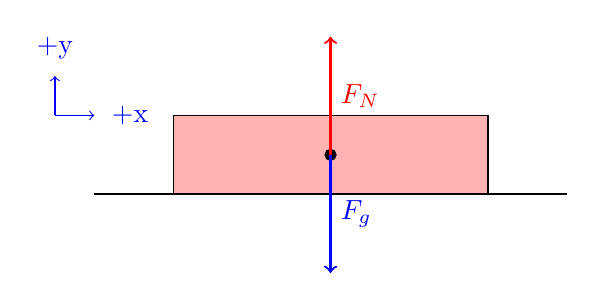
\begin{tikzpicture}
			
			% Draw the book
			\draw[fill=red!30] (0,0) rectangle (4,1); % The book as a rectangle
			%	\node at (2,0.5) {}; % Label for the book
			
			% Draw the table (optional)
			\draw[thick] (-1,0) -- (5,-0); % Table surface
			
			% Center of Mass (dot in the middle)
			\filldraw[black] (2,0.5) circle (2pt); % Dot for the center of mass
			%		\node at (2.5,0.8) {};
			
			% Draw the forces acting on the book
			% Normal force (upward)
			\draw[->, thick, red] (2,0.5) -- (2,2) node[midway, right] {$F_N$};
			
			% Weight (downward)
			\draw[->, thick, blue] (2,0.5) -- (2,-1) node[midway, right] {$F_g$};
			
			% Add labels for the diagram
			%	\node at (2,-2) {Free Body Diagram of a book on a table};
			%Draw the coordinate system
			\draw[->,blue] (-1.5,1) -- (-1.5,1.5);
			\node at (-1.5,1.6) [above,blue] {+y};
			
			\draw[->,blue] (-1.5,1) -- (-1,1);
			\node at (-0.9,1) [right,blue] {+x};
			
		\end{tikzpicture}
	\end{center}
	
	In this diagram, the normal force and the gravitational force are balanced.  Thus, the object remains at rest, according to Newton's 1st Law.  
	
\end{mdframed}	



\begin{mdframed}[backgroundcolor=blue!10!white]
	\begin{center}

		
		\textbf{Example \thesection.2}	
	\end{center}
	
	\textbf{Problem: } As a person walks through an airport, she pulls a suitcase at a constant speed using a strap at a 25 degree angle above horizontal.  Friction is significant.  Draw a free body diagram of the situation.
	\vspace{0.1in}
	
	\textbf{Solution:} 
	The diagram should look as follows:
	
	\begin{center}
		
		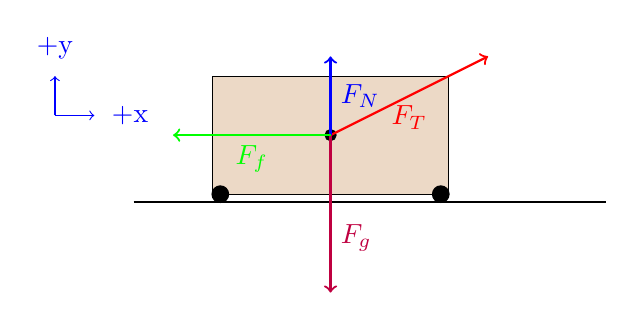
\begin{tikzpicture}
			
			% Draw the suitcase
			\draw[fill=brown!30] (0,0) rectangle (3,1.5); % Suitcase as a rectangle
			%	\node at (1.5,0.75) {Suitcase}; % Label for suitcase
			\draw[fill=black] (0.1,0) circle (3 pt); % wheel 1
			\draw[fill=black] (2.9,0) circle (3 pt); % wheel 2
			
			
			% Draw the ground (optional)
			\draw[thick] (-1,-0.1) -- (5,-0.1); % Ground line
			
			% Center of mass (dot in the middle)
			\filldraw[black] (1.5,0.75) circle (2pt); % Dot for center of mass
			
			% Draw the forces acting on the suitcase
			% Tension force (pulling force at 25-degree angle)
			\draw[->, thick, red] (1.5,0.75) -- ++(2,1) node[midway, below] {$F_T$};
			%\node at (1.6,0.75) [right,red] {$25^\circ$}; % Angle of the tension force
			
			% Normal force (upward)
			\draw[->, thick, blue] (1.5,0.75) -- ++(0,1) node[midway, right] {$F_N$};
			
			% Weight force (downward)
			\draw[->, thick, purple] (1.5,0.75) -- (1.5,-1.25) node[midway, below right] {$F_g$};
			
			% Friction force (leftward)
			\draw[->, thick, green] (1.5,0.75) -- (-0.5,0.75) node[midway, below] {$F_f$};
			
			% Add labels for the diagram
			%	\node at (1.5,-1.8) {Free Body Diagram of a suitcase being pulled at a 25-degree angle};
			
			
			%Draw the coordinate system
			\draw[->,blue] (-2,1) -- (-2,1.5);
			\node at (-2,1.6) [above,blue] {+y};
			
			\draw[->,blue] (-2,1) -- (-1.5,1);
			\node at (-1.4,1) [right,blue] {+x};
		\end{tikzpicture}
		
		
		
	\end{center}
	
	In this diagram, the sum of the forces that act in the x-direction (friction, and the x-component of tension) must equal zero to ensure the suitcase maintains a constant horizontal speed.  In addition, the forces that act in the y-direction (Gravity, Normal Force, and the Y-component of tension) must sum to equal zero as well so that the suitcase does not accelerate vertically.  
	
\end{mdframed}	


\newpage
	\section{Newton's First Law} \index{Newton's First Law} \index{Law of Inertia}
	\begin{tabular}{p{.75in} p{4.5in} p{.75in}}
		 & \textit{Corpus omne perseverare in statu suo quiescendi vel movendi uniformiter in directum, nisi quatenus a viribus impressis cogitur statum illum mutare.} &  \\
		  & & \\
		 & \textit{Every body continues in its state of being at rest or moving uniformly in a direction, except insofar as it is compelled to change its state by means of an imparted force. } & \\
		 & & \\

		&  -- Newton, Isaac.  \textit{Philosophiae Naturalis Principia Mathematica}.  tr. J. Williamson & \\
		& & \\
	\end{tabular}

	

	
  You may have heard Sir Isaac Newton's first law of physics stated in different ways than the above.  Often in grade school, students are taught a phrase beginning with ``objects in motion...''.  	Sometimes this law is called the ``Law of Inertia''.   This is a very basic understanding of the complexity of this law.  In fact, all non-accelerating systems are governed by this law.  As long as the vector sum of the forces upon an object is zero, the object will continue in a state of uniform motion (remaining at rest is a type of uniform motion) until something causes the equilibrium of the system to be lost.  
	Likewise, if an object is known to have an acceleration of zero, we can state that the vector sum of the forces is equal to zero.  We can use this law to characterize non-accelerating systems:
	
				\begin{mdframed}[backgroundcolor=orange!20!white]
		\begin{equation}
			\Sigma \vec{F} = 0  
			\label{eqn:newtonsfirst}
		\end{equation}
	\end{mdframed}

\newpage

	
	\section{Newton's Second Law}
	\index{Newton's Second Law}
		\begin{tabular}{p{.75in} p{4.5in} p{.75in}}
		& \textit{Mutationem motus proportionalem esse vi motrici impressae, et fieri secundum lineam rectam qua vis illa imprimitur.} &  \\
		& & \\
		& \textit{The change in motion is proportional to the amount of force of motion imparted, and according to the straight line made by the force impressed. } & \\ 
		& & \\
		 & {-Newton, Isaac.  \textit{Philosophiae Naturalis Principia Mathematica}.  tr. J. Williamson} & \\		
		 	& & \\
	\end{tabular}

Newton's Second Law describes objects and systems that have a constant acceleration.  The vector sum of the forces on an object is equal to the object's mass times its acceleration:

				\begin{mdframed}[backgroundcolor=orange!20!white]
	\begin{equation}
		\Sigma \vec{F} = m \vec{a}  
		\label{eqn:newtonssecond}
	\end{equation}
\end{mdframed}
	
	It should be noted that forces are vectors.  Thus, when forces are combined, their directions should be taken into account.  The direction of the net force is always in the same direction as the acceleration of the object. 
	
	It should also be noted that if all the forces on an object cancel, the acceleration of the object will be zero - which means that the first law is just a special case of the second law when $\Sigma F = 0 N$.
	
	Often, if the forces on an object of known mass can be determined, the acceleration of the object can also be determined.  The acceleration found using Newton's second law can then be used in kinematic equations to determine other important quantities. 
	
	 
	
	\section{Newton's Third Law}
	\index{Newton's Third Law}
		\begin{tabular}{p{.75in} p{4.5in} p{.75in}}
		&  &  \\
		& & \\
		& \textit{Actioni contrariam semper et aequalem esse reactionem: sive corporum duorum actiones in se mutuo semper esse aequales et in partes contrarias dirigi. } & \\
		& & \\
		& \textit{For an action there is always an equal and opposite reaction: or the two bodies on each other are always equal and in opposite directions. } & \\
		& & \\
		 & {-Newton, Isaac.  \textit{Philosophiae Naturalis Principia Mathematica}.  tr. J. Williamson} & \\
		
	\end{tabular}
	
	\section{Applications of Newton's Laws}
		\subsection{Friction}
		\index{Friction}
		\textbf{Friction} occurs whenever two surfaces are in contact, and it is a force that has two effects.  
		\begin{itemize}
			\item Friction always opposes the motion of an object, or even the tendency to move.
			\item Friction dissipates energy into heat.
		\end{itemize}
		
		\index{Friction, static} \index{Friction, kinetic}
		There are two types of friction that one should know about: \textbf{static friction} and \textbf{kinetic friction}.  Static friction is present when two surfaces are in contact, but not sliding.  Kinetic friction is occurs when two surfaces are in contact and sliding past each other.  One should note that when an object is rolling, there is static friction between the outer edge of the wheel and the surface it is rolling on, whereas static or kinetic friction may be present where the wheel is connected to the axle, depending on the type of joint that is used.  
		
		\index{Coefficient of Friction}
		The \textbf{coefficient of static friction}  and the \textbf{coefficient of kinetic friction}, symbolized by $\mu_s$ and $\mu_k$ respectively, measure how hard it is to slide two surfaces past each other.  A surface that is very slippery will have low coefficients of friction, whereas surfaces that grip each other well will very high coefficients of friction. A perfectly frictionless surface would have a coefficient of friction of 0.  Some examples of coefficients of friction can be found in \color{red} insert reference here\color{black}.  One should also note that the coefficients of friction are unitless.  
		
		To calculate the force of static friction, the following formula is used:
		\index{Static Friction}
		\index{Friction, static}
		\begin{mdframed}[backgroundcolor=orange!20!white]
			\begin{equation}
				|F_f| \leq \mu_s |F_N|  
				\label{eqn:frictionstatic}
			\end{equation}
		\end{mdframed}
	
	The force of kinetic friction can be calculated by using this formula:
			\index{Friction, kinetic}
			\index{Kinetic Friction}
			\begin{mdframed}[backgroundcolor=orange!20!white]
		\begin{equation}
			|F_f| = \mu_k |F_N|  
			\label{eqn:frictionkinetic}
		\end{equation}
	\end{mdframed}
		
		
		
		\subsection{Inclined Planes}
		\index{Inclined Plane}
		
		
		\newcommand{\angler}{30}
		\begin{figure}[H]
			\centering
		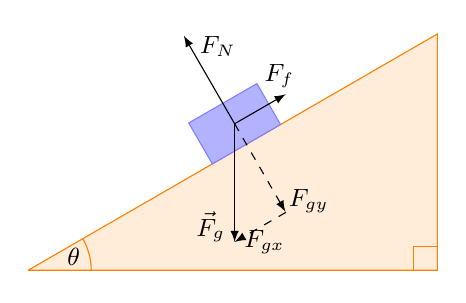
\begin{tikzpicture} [font = \small]
			
			% triangle:
			\draw [draw = orange, fill = orange!15] (0,0) coordinate (O) -- (\angler:6)
			coordinate [pos=.45] (M) |- coordinate (B) (O);
			
			% angles:
			\draw [draw = orange] (O) ++(.8,0) arc (0:\angler:0.8) 
			node [pos=.4, left] {$\theta$};
			\draw [draw = orange] (B) rectangle ++(-0.3,0.3);
			
			\begin{scope} [-latex,rotate=\angler]
				
				% Object (rectangle)
				\draw [fill = blue!30,
				draw = blue!50] (M) rectangle ++ (1,.6);
				
				% Weight Force and its projections
				\draw [dashed] (M) ++ (.5,.3) coordinate (MM) -- ++ (0,-1.29)
				node [very near end, right] {$F_{gy}$};
				
				\draw [dashed] (3.2,-1) -- ++ (-0.75,0) 
				node [right] {$F_{gx}$};
				
				\draw (MM) -- ++ (-\angler-90:1.5)
				node [very near end,left ] {$\vec{F}_g$};
				
				% Normal Force
				\draw (MM) -- ++ (0,1.29)
				node [very near end, right] {$F_N$};
				
				% Frictional Force
				\draw (MM) -- ++ (0.75,0)
				node [very near end, above] {$F_f$};
				
			\end{scope}
			
		\end{tikzpicture} 
		\caption{An inclined plane}
				\end{figure}
		
		
		
		\subsection{Elevators}
		\index{Elevator}
		\index{Apparent Weight}
		
		
		
		
		\subsection{Pulleys and Atwood Machines}
		\index{Atwood Machine}
		


	


